\documentclass[11pt]{amsart}
\usepackage[T1]{fontenc}
\usepackage{lmodern}
\usepackage{amsmath,amssymb,amsthm}
\usepackage{graphicx}
\usepackage{booktabs}
\usepackage[margin=1.15in]{geometry}
\usepackage{microtype}
\usepackage[hidelinks]{hyperref}
\emergencystretch=3em

\newcommand{\NBOUND}{339\,110\,855}
\newcommand{\NTOT}{4\,115\,897}
\newcommand{\DMAX}{227\,932\,027}
\newcommand{\HDMAX}{996}
\newcommand{\NFUND}{103\,077\,319}
\newcommand{\MINL}{0.198814}
\newcommand{\MINLD}{-991\,027}
\newcommand{\TIMECOUNT}{15 minutes}


\newtheorem{theorem}{Theorem}[section]
\newtheorem{lemma}[theorem]{Lemma}
\newtheorem{proposition}[theorem]{Proposition}
\newtheorem{corollary}[theorem]{Corollary}
\theoremstyle{definition}
\newtheorem{definition}[theorem]{Definition}
\theoremstyle{remark}
\newtheorem{remark}[theorem]{Remark}

\newcommand{\Lam}{\Lambda_\chi}
\renewcommand{\Re}{\operatorname{Re}}
\renewcommand{\Im}{\operatorname{Im}}

\title{Class Numbers up to Ten Thousand and Zero-Free Half-Planes}
\hypersetup{pdftitle={Class Numbers up to Ten Thousand and Zero-Free Half-Planes},pdfauthor={Deep Bhattacharjee}}

\author{Deep Bhattacharjee}
\address{Formerly, Electro-Gravitational Space Propulsion Laboratory (EGSPL), Bhubaneswar, Odisha 751030, India}
\address{Formerly, University of Calcutta (Heramba Chandra College), 23/49 Gariahat Road, Golpark, Kolkata 700029, West Bengal, India}
\email{d.bhattacharjee@erl-forschung.de}
\email{itsdeep@live.com}
\email{egspl@proton.me}
\urladdr{https://orcid.org/0000-0003-0466-750X}
\urladdr{https://github.com/creelie}
\thanks{Corresponding author: Deep Bhattacharjee, d.bhattacharjee@erl-forschung.de. For matters concerning the code and data: egspl@proton.me (GitHub: creelie).}

\subjclass[2020]{Primary 11R29, 11M20; Secondary 11R11, 11Y40}
\keywords{class number problem, Dirichlet $L$-functions, zero-free half-plane, Siegel zeros, imaginary quadratic fields}



\begin{document}
\begin{abstract}
We prove, with every constant explicit, that a zero-free half-plane $\Re s>B$ for all Dirichlet $L$-functions gives two-sided bounds for $L(1,\chi)$ of Littlewood's shape with $\log\log q$ multiplied by $1/(1-B)$. For $B=7/8$ these read $0.725/(8\log\log q-4.15)\le|L(1,\chi)|\le 2.27\,(8\log\log q-4.15)$ for conductors $q\ge 2^{40}$. Under this hypothesis every imaginary quadratic field of class number at most $10\,798$ has discriminant below $2^{40}$, so its class number problem is solved by the existing unconditional tables, and we count the fields of each class number up to $1000$. Without any hypothesis, Tatuzawa's theorem gives the same conclusion for class numbers up to $2900$ with at most one possible exceptional field.
\end{abstract}
\maketitle

\section{Introduction}

Gauss conjectured in the \emph{Disquisitiones Arithmeticae} that for each $h$ only finitely many negative discriminants have class number $h$, and he gave the lists he believed complete for small $h$. The class number problem asks for these lists. Heilbronn proved finiteness, Siegel's theorem $L(1,\chi_d)\gg_\varepsilon |d|^{-\varepsilon}$ made it quantitative but ineffective \cite{Sie35}, and the case $h=1$ was settled by Heegner \cite{Hee52}, Baker \cite{Bak66} and Stark \cite{Sta67}. Goldfeld's reduction \cite{Gol85} to an $L$-function with a zero of order three at the centre, supplied by Gross and Zagier \cite{GZ86}, gave an effective but very small lower bound for $h(d)$, and Watkins \cite{Wat04} used it to determine every field with $h(d)\le 100$.\footnote{The Goldfeld--Gross--Zagier bound grows only like $\log|d|$, up to a factor depending on the prime divisors of $d$; Watkins combined it with extensive computations.}

The obstruction to doing better is the possible Siegel zero, a real zero of $L(s,\chi_d)$ very close to $s=1$. A zero-free half-plane for all Dirichlet $L$-functions removes it. Proofs of such a half-plane have recently been announced: zero-freeness in $\Re s>7/8$ \cite{OAI-QRH}, with a Lean formalisation of its Dirichlet part \cite{OAI-family}, the weaker region $\Re s>11/12$ by a separate argument \cite{OAI-1112}, and an improvement of $7/8$ to $0.874957\ldots$ by Liu \cite{Liu26}. These works have not yet been refereed, so in this paper the half-plane is a hypothesis, named below, and each theorem states it. A half-plane gives $L(1,\chi)\gg 1/\log\log q$ with an unstated constant. We make every constant explicit and certify it, and combine the result with the unconditional tabulation of Mosunov and Jacobson \cite{MJ16}; the outcome is the class number problem in a range a hundred times larger than that of Watkins, under the half-plane hypothesis.

For $\tfrac12\le B<1$ we write
\[
\mathrm{H}(B):\qquad L(s,\chi)\neq0 \ \text{ for every primitive Dirichlet character }\chi\ \text{and every }s \text{ with } \Re s>B .
\]
The announced theorem of \cite{OAI-QRH} is $\mathrm{H}(7/8)$. Theorems~\ref{thm:general} and~\ref{thm:uniform} below are unconditional implications from $\mathrm{H}(B)$ to explicit bounds; the hypothesis enters only through them.

\begin{theorem}\label{thm:main}
Assume $\mathrm{H}(7/8)$. Let $\chi$ be a primitive Dirichlet character of conductor $q\ge 2^{40}$. Then
\[
\frac{0.725}{8\log\log q-4.15}\ \le\ |L(1,\chi)|\ \le\ 2.27\,\bigl(8\log\log q-4.15\bigr).
\]
\end{theorem}

Under the generalised Riemann hypothesis Littlewood \cite{Lit28} proved that $|L(1,\chi)|$ lies between constant multiples of $(\log\log q)^{-1}$ and $\log\log q$. Theorem~\ref{thm:main} is the case $B=7/8$ of Theorem~\ref{thm:uniform}, which gives such bounds under $\mathrm{H}(B)$ for every $B<1$ with the factor $1/(1-B)$ in front of $\log\log q$. For the half-plane $\Re s>11/12$ alone it gives $0.714/(12\log\log q-8.55)\le|L(1,\chi)|$.

For a fundamental discriminant $d<-4$ the class number formula reads $h(d)=\sqrt{|d|}\,L(1,\chi_d)/\pi$, where $\chi_d$ is the primitive real character of conductor $|d|$ \cite[Chapter 6]{Dav80}.

\begin{theorem}\label{thm:h}
Assume $\mathrm{H}(7/8)$. Then every fundamental discriminant $d<-2^{40}$ has $h(d)\ge 10\,799$. Under the weaker hypothesis $\mathrm{H}(11/12)$, $h(d)\ge 7\,612$.
\end{theorem}

Mosunov and Jacobson \cite{MJ16} computed, without any hypothesis, the class group of every imaginary quadratic field with $|d|<2^{40}$; the smallest value of $L(1,\chi_d)$ in that range is $0.17070\ldots$, attained at $d=-107\,415\,709\,003$.

\begin{corollary}\label{cor:cnp}
Assume $\mathrm{H}(7/8)$, and let $1\le h\le 10\,798$. Every imaginary quadratic field of class number $h$ has
\[
|d|\ \le\ \Bigl(\frac{\pi h}{0.1706}\Bigr)^{2}\ <\ 2^{40}.
\]
In particular every such field has $|d|<3.4\cdot10^{10}$ when $h\le 10^4$, and the complete list of fields of class number $h$ is the list contained in the tabulation of \cite{MJ16}.
\end{corollary}

\begin{proof}
By Theorem~\ref{thm:h}, $|d|<2^{40}$. By \cite{MJ16}, $L(1,\chi_d)\ge 0.1706$ in that range, so $h=\sqrt{|d|}\,L(1,\chi_d)/\pi\ge 0.1706\sqrt{|d|}/\pi$ (the fields with $d=-3,-4$ have $h=1$ and satisfy the bound). For $h\le 10\,798$ the right-hand side of the display is $\le 3.96\cdot10^{10}<2^{40}=1.0995\cdot10^{12}$.
\end{proof}

For $h\le 1000$ the bound is $|d|\le 3.3911\cdot 10^{8}$, small enough to count reduced forms directly.

\begin{theorem}\label{thm:list}
Assume $\mathrm{H}(7/8)$. For $1\le h\le 1000$ the imaginary quadratic fields of class number $h$ are exactly those with $|d|\le \NBOUND$ and $h(d)=h$. There are $\NTOT$ of them; the largest $|d|$ is $\DMAX$, of class number $\HDMAX$. The number $F(h)$ of fields of class number $h$ and the largest $|d|$ for each $h$ are given in Appendix~\ref{app:data} for selected $h$ and in full in the ancillary data.
\end{theorem}

Without any hypothesis on zeros, the same tables decide the class number problem in a smaller range, up to a single field that cannot be excluded by present methods.

\begin{theorem}\label{thm:uncond}
There is at most one fundamental discriminant $d^*<-2^{40}$ such that every fundamental discriminant $d<-2^{40}$ with $d\neq d^*$ satisfies $h(d)\ge 2901$. Consequently, for $1\le h\le 2900$ every imaginary quadratic field of class number $h$, with the possible exception of the single field $\mathbb Q(\sqrt{d^*})$, has $|d|\le(\pi h/0.1706)^2$ and appears in the tabulation of \cite{MJ16}; in particular the counts of Theorem~\ref{thm:list} are unconditionally complete apart from at most one field.
\end{theorem}

Theorem~\ref{thm:uncond} is proved in Section~\ref{sec:uncond}. It uses no zero-free region; the price is the possible exception, which is the Siegel zero in another form.

For $h\le100$ the counts and the largest discriminants agree with those of Watkins \cite{Wat04}; his tables stop at $h=100$.

\begin{figure}[t]
\centering
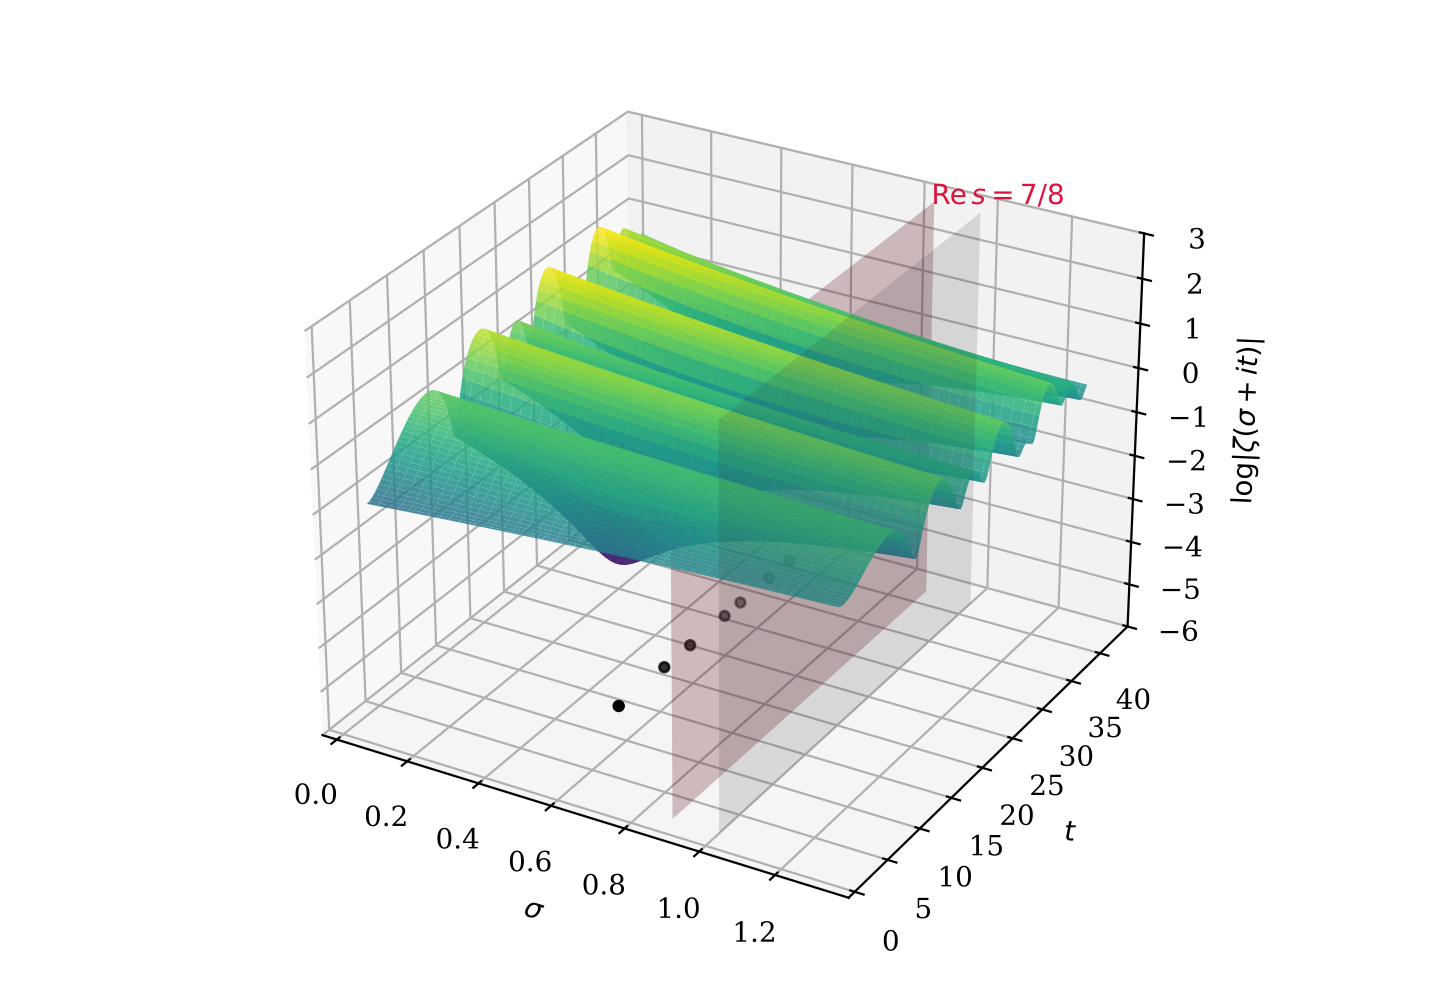
\includegraphics[width=0.86\textwidth]{figures/fig_strip.png}
\caption{The surface $\log|\zeta(\sigma+it)|$ over the critical strip, with the plane $\sigma=7/8$ and the first zeros on the line $\sigma=1/2$. The theorems of this paper use only that no zero of any Dirichlet $L$-function lies to the right of the plane.}
\label{fig:strip}
\end{figure}

\subsection*{Method}
The proof of Theorem~\ref{thm:main} is a smoothed explicit formula. Integrating the formula for $\sum\Lam(n)n^{-1-u}\log(x/n)$ over $u\in[0,\infty)$ produces $\log L(1,\chi)$ itself on one side and, on the other, a sum over zeros in which each zero $\rho$ contributes at most $x^{\beta-1}/(|\rho-1|^2\log x)$. Taking the difference of two such formulas at $x$ and $y$ leaves a prime sum with a weight that is $1$ up to $y$ and decays linearly in $\log n$ up to $x$ (Figure~\ref{fig:method}). Under $\mathrm{H}(B)$ every term $x^{\beta-1}$ is at most $x^{B-1}$, the sum $\sum_\rho|\rho-1|^{-2}$ is $O(\log q)$ by the Hadamard product, and the choice $y=(\log q)^{1/(1-B)}$ makes the zero contribution bounded. The prime sum is then bounded with the explicit estimates of Rosser and Schoenfeld \cite{RS62}. Every constant is evaluated in interval arithmetic \cite{Joh17}.

\subsection*{Organisation}
Section~\ref{sec:explicit} proves the explicit formula and its integrated form, Section~\ref{sec:zeros} bounds the zeros, Section~\ref{sec:primes} the primes, and Section~\ref{sec:proofs} proves Theorems~\ref{thm:main} and~\ref{thm:h}. Section~\ref{sec:uncond} proves Theorem~\ref{thm:uncond} and Section~\ref{sec:forms} proves Theorem~\ref{thm:list}. Appendix~\ref{app:contour} contains the contour argument, Appendix~\ref{app:numerics} the certified constants, Appendix~\ref{app:data} the data.

\section{The integrated explicit formula}\label{sec:explicit}

Throughout, $\chi$ is a primitive character modulo $q\ge3$, $a\in\{0,1\}$ is defined by $\chi(-1)=(-1)^a$, $\Lam(n)=\Lambda(n)\chi(n)$, and $\rho=\beta+i\gamma$ runs over the nontrivial zeros of $L(s,\chi)$ with multiplicity. They satisfy $0<\beta<1$, and $\sum_\rho|\rho|^{-2}<\infty$ \cite[Chapter 12]{Dav80}. The trivial zeros are $s=-2k-a$, $k\ge0$.

\begin{lemma}\label{lem:explicit}
For $x>1$ and $u\ge0$,
\begin{multline}\label{eq:explicit}
\sum_{n\le x}\frac{\Lam(n)}{n^{1+u}}\log\frac xn
=-\frac{L'}{L}(1+u,\chi)\log x-\Bigl(\frac{L'}{L}\Bigr)'(1+u,\chi)\\
-\sum_\rho\frac{x^{\rho-1-u}}{(\rho-1-u)^2}
-\sum_{k\ge0}\frac{x^{-2k-a-1-u}}{(2k+a+1+u)^2}.
\end{multline}
Both sums converge absolutely.
\end{lemma}

\begin{proof}
Put $s=1+u$. For $y>0$ and $c>0$ one has $\frac1{2\pi i}\int_{(c)}y^w w^{-2}\,dw=\max(\log y,0)$, with absolute convergence. Since $-\frac{L'}{L}(s+w,\chi)=\sum\Lam(n)n^{-s-w}$ converges absolutely on $\Re w=1$, termwise integration gives
\[
\sum_{n\le x}\frac{\Lam(n)}{n^{s}}\log\frac xn=\frac1{2\pi i}\int_{(1)}\Bigl(-\frac{L'}{L}(s+w,\chi)\Bigr)\frac{x^w}{w^2}\,dw .
\]
The integrand is meromorphic. At $w=0$ it has a double pole with residue $-\frac{L'}{L}(s,\chi)\log x-(\frac{L'}{L})'(s,\chi)$; at $w=\rho-s$ a pole with residue $-x^{\rho-s}/(\rho-s)^2$ times the multiplicity of $\rho$; at $w=-2k-a-s$ a pole with residue $-x^{-2k-a-s}/(2k+a+s)^2$. Moving the line of integration to $-\infty$ through a sequence of rectangles on which $L'/L$ is controlled (Appendix~\ref{app:contour}) proves \eqref{eq:explicit}. Absolute convergence follows from $|\rho-s|\ge|\rho-1|\gg|\rho|$ and $\sum|\rho|^{-2}<\infty$.\footnote{The square of $w$ in the kernel $x^w/w^2$ is what makes the sum over zeros converge absolutely, with no truncation in height.}
\end{proof}

Integration of \eqref{eq:explicit} over $u$ removes the derivative and leaves $\log L(1,\chi)$. Here $\log L(s,\chi)=\sum_{n\ge2}\Lam(n)n^{-s}/\log n$ for $\Re s>1$, continued along the real segment to $s=1$; this is possible because $L(1+u,\chi)\neq0$ for $u\ge0$.

\begin{proposition}\label{prop:integrated}
For $x>1$ put
\[
V(x)=\sum_{2\le n\le x}\frac{\Lam(n)}{n\log n}\log\frac xn .
\]
Then
\[
V(x)=\log L(1,\chi)\,\log x+\frac{L'}{L}(1,\chi)-\sum_\rho I_\rho(x)-T(x),
\]
where
\[
|I_\rho(x)|\le\frac{x^{\beta-1}}{|\rho-1|^2\log x},\qquad |T(x)|\le \frac{\pi^2}{8\,x\log x}.
\]
\end{proposition}

\begin{proof}
Integrate \eqref{eq:explicit} over $u\in[0,\infty)$. On the left, $\int_0^\infty n^{-1-u}\,du=1/(n\log n)$ for $n\ge2$, which gives $V(x)$. On the right, $\int_0^\infty-\frac{L'}{L}(1+u,\chi)\,du=\log L(1,\chi)$ and $\int_0^\infty-(\frac{L'}{L})'(1+u,\chi)\,du=\frac{L'}{L}(1,\chi)$, since $\log L(1+u,\chi)$ and $\frac{L'}{L}(1+u,\chi)$ tend to $0$ as $u\to\infty$. The zero term is
\[
I_\rho(x)=\int_0^\infty\frac{x^{\rho-1-u}}{(\rho-1-u)^2}\,du .
\]
Since $1-\beta+u\ge1-\beta>0$, we have $|\rho-1-u|^2=(1-\beta+u)^2+\gamma^2\ge|\rho-1|^2$, hence
\[
|I_\rho(x)|\le\frac{x^{\beta-1}}{|\rho-1|^2}\int_0^\infty x^{-u}\,du=\frac{x^{\beta-1}}{|\rho-1|^2\log x}.
\]
In the same way the $k$-th trivial term is at most $x^{-2k-a-1}/((2k+a+1)^2\log x)$, and
$\sum_{k\ge0}(2k+a+1)^{-2}\le\sum_{k\ge0}(2k+1)^{-2}=\pi^2/8$. Interchanging the integral with the sums over zeros is justified by the bounds just proved and $\sum_\rho|\rho-1|^{-2}<\infty$.
\end{proof}

Subtracting the formula at $y$ from the formula at $x$ eliminates the unknown constant $\frac{L'}{L}(1,\chi)$.

\begin{corollary}\label{cor:difference}
Let $1<y<x$, $\lambda=x/y$ and $\ell=\log\lambda$. Define $w(n)=1$ for $n\le y$, $w(n)=\log(x/n)/\ell$ for $y<n\le x$, and $w(n)=0$ for $n>x$. Then
\begin{equation}\label{eq:difference}
\log L(1,\chi)=\sum_{n\ge2}\frac{\Lam(n)\,w(n)}{n\log n}+\theta\,\mathcal E,\qquad |\theta|\le1,
\end{equation}
where
\[
\mathcal E=\frac1\ell\Bigl[\Bigl(\frac{x^{\beta^*-1}}{\log x}+\frac{y^{\beta^*-1}}{\log y}\Bigr)\sum_\rho\frac1{|\rho-1|^2}+\frac{\pi^2}{8}\Bigl(\frac1{x\log x}+\frac1{y\log y}\Bigr)\Bigr]
\]
and $\beta^*=\sup_\rho\beta$.
\end{corollary}

\begin{proof}
For $n\le y$ the difference $\log(x/n)-\log(y/n)$ equals $\ell$; for $y<n\le x$ only $\log(x/n)$ is present. Hence $V(x)-V(y)=\ell\sum\Lam(n)w(n)/(n\log n)$. Proposition~\ref{prop:integrated} gives $V(x)-V(y)=\ell\log L(1,\chi)-\sum_\rho(I_\rho(x)-I_\rho(y))-(T(x)-T(y))$, and the bounds there with $x^{\beta-1}\le x^{\beta^*-1}$ give the claim.
\end{proof}

\begin{figure}[t]
\centering
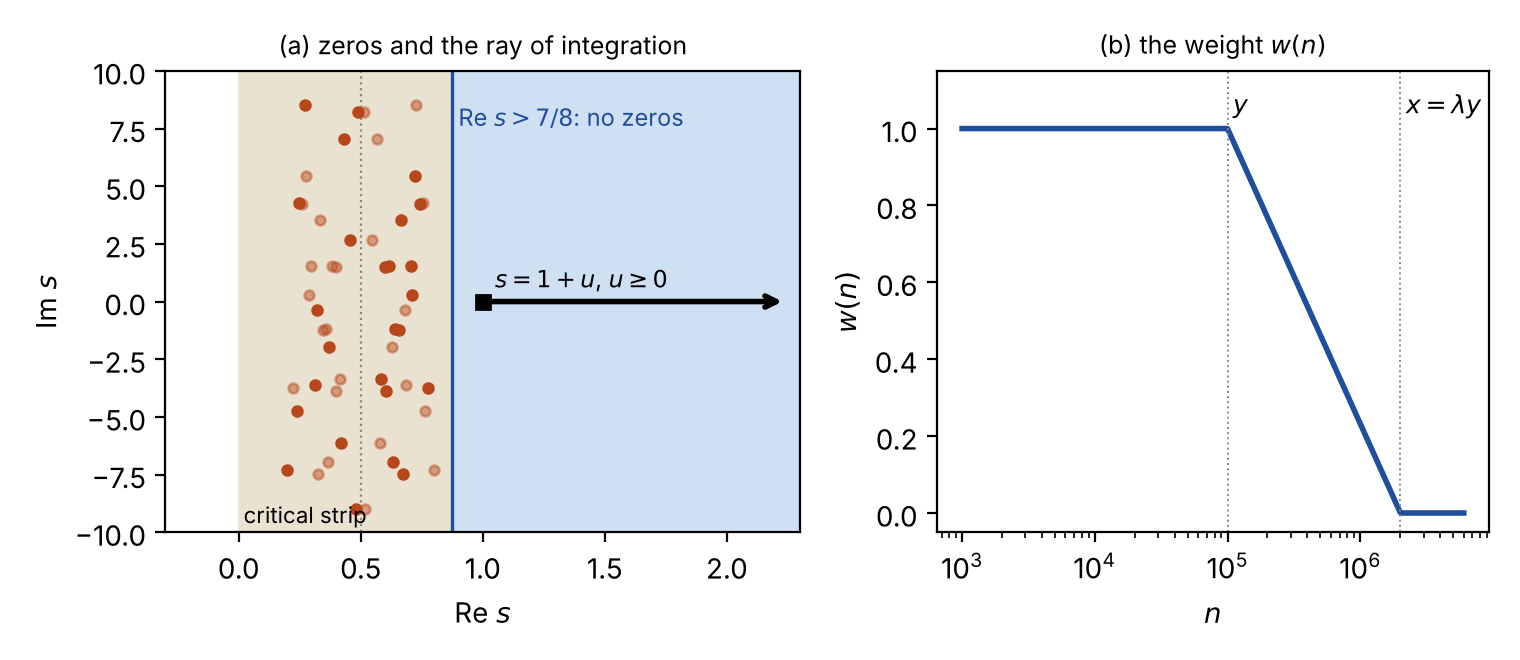
\includegraphics[width=0.95\textwidth]{figures/fig_method.png}
\caption{(a) Under $\mathrm H(7/8)$ every zero lies in $\beta\le 7/8$; the formula is integrated along the ray $s=1+u$. (b) The weight of Corollary~\ref{cor:difference}: equal to $1$ up to $y$ and linear in $\log n$ between $y$ and $x=\lambda y$.}
\label{fig:method}
\end{figure}

\section{The sum over zeros}\label{sec:zeros}

\begin{lemma}\label{lem:zerosum}
Assume that every zero of $L(s,\chi)$ has $\beta\le B$, where $\tfrac12\le B<1$. Then for every $u>0$,
\[
\sum_\rho\frac1{|\rho-1|^2}\ \le\ S(q,u,B):=\frac{1+u-B}{(1-B)^2}\Bigl(\frac12\log\frac q\pi+\frac12\psi\Bigl(1+\frac u2\Bigr)-\frac{\zeta'}{\zeta}(1+u)\Bigr),
\]
where $\psi=\Gamma'/\Gamma$.
\end{lemma}

\begin{proof}
Let $\sigma=1+u$. The Hadamard product \cite[Chapter 12]{Dav80} gives
\[
\frac{L'}{L}(s,\chi)=-\frac12\log\frac q\pi-\frac12\psi\Bigl(\frac{s+a}2\Bigr)+b(\chi)+\sum_\rho\Bigl(\frac1{s-\rho}+\frac1\rho\Bigr),\qquad \Re b(\chi)=-\sum_\rho\Re\frac1\rho,
\]
so that, at $s=\sigma$,
\begin{equation}\label{eq:hadamard}
\sum_\rho\frac{\sigma-\beta}{|\sigma-\rho|^2}=\frac12\log\frac q\pi+\frac12\psi\Bigl(\frac{\sigma+a}2\Bigr)+\Re\frac{L'}{L}(\sigma,\chi).
\end{equation}
Since $\psi$ is increasing, $\psi((\sigma+a)/2)\le\psi(1+u/2)$, and $|\frac{L'}{L}(\sigma,\chi)|\le\sum\Lambda(n)n^{-\sigma}=-\frac{\zeta'}{\zeta}(\sigma)$. On the other side, $\sigma-\beta\ge1-\beta>0$ gives $|\sigma-\rho|^2\le((\sigma-\beta)/(1-\beta))^2|1-\rho|^2$, that is,
\[
\frac1{|1-\rho|^2}\le\frac{\sigma-\beta}{(1-\beta)^2}\cdot\frac{\sigma-\beta}{|\sigma-\rho|^2}.
\]
The function $\beta\mapsto(\sigma-\beta)/(1-\beta)^2$ is increasing on $(-\infty,1)$, because its derivative is $(1-\beta)^{-3}(2\sigma-1-\beta)>0$, so it is at most $(\sigma-B)/(1-B)^2$. Summing over $\rho$ and using \eqref{eq:hadamard} proves the lemma.
\end{proof}

\begin{remark}
The factor $(1+u-B)/(1-B)^2$ is where the width of the zero-free region enters. Under the Riemann hypothesis for $L(s,\chi)$ it would be $4(1/2+u)$, and the bound would be the classical $\sum_\rho|\rho-1|^{-2}=\sum_\rho 1/(1/4+\gamma^2)\sim\log q$.
\end{remark}

\section{The sum over primes}\label{sec:primes}

Let $B_1=0.2614972128\ldots$ be Mertens' constant, so that $\sum_{p\le t}1/p=\log\log t+B_1+o(1)$, let $\gamma$ be Euler's constant, and put
\[
G(y)=\sum_{p\le y}\Bigl(\frac1p-\log\Bigl(1+\frac1p\Bigr)\Bigr),\qquad F(v)=v\log v-v+B_1v-\frac1{2v}.
\]
The terms of $G$ are positive, so $G$ increases; $G(10^6)=0.1819818165\ldots$ and $G(\infty)=0.18198\ldots$.

\begin{lemma}\label{lem:primes}
Let $286\le y<x$, $\ell=\log(x/y)$, and let $M$ be the sum in \eqref{eq:difference}. Put $W=(F(\log x)-F(\log y))/\ell$. Then
\[
-W+G(y)-\frac3{\sqrt y}\ \le\ \Re M\ \le\ W+\gamma-B_1+\frac3{\sqrt y}.
\]
\end{lemma}

\begin{proof}
Only prime powers contribute, and $\Lambda(p^k)/(p^k\log p^k)=1/(kp^k)$. Since $w(p^k)=1$ when $p^k\le y$, we can write
\[
M=\sum_{p\le y}-\log\Bigl(1-\frac{\chi(p)}p\Bigr)+\sum_{y<p\le x}\frac{\chi(p)w(p)}p+R,
\]
where
\[
R=\sum_{\substack{p\le y,\ k\ge2\\ p^k>y}}\frac{\chi(p)^k(w(p^k)-1)}{kp^k}+\sum_{\substack{p>y\\ k\ge2}}\frac{\chi(p)^kw(p^k)}{kp^k}.
\]
Since $0\le w\le1$, we have $|R|\le\frac12\sum_p\sum_{k\ge2,\,p^k>y}p^{-k}$. For fixed $p$ let $k_0$ be the least $k\ge2$ with $p^k>y$; the inner sum is at most $p^{-k_0}p/(p-1)\le2p^{-k_0}$. If $p\le\sqrt y$ then $p^{-k_0}<1/y$, and there are at most $\sqrt y$ such primes; if $p>\sqrt y$ then $k_0=2$. Hence
\[
|R|\le\frac{\sqrt y}{y}+\sum_{m>\sqrt y}\frac1{m^2}\le\frac1{\sqrt y}+\frac1{\sqrt y-1}\le\frac3{\sqrt y}.
\]
For the lower bound, $\Re(-\log(1-\chi(p)/p))=-\log|1-\chi(p)/p|\ge-\log(1+1/p)$ and $\Re\chi(p)w(p)/p\ge-w(p)/p$. Thus
\[
\Re M\ge G(y)-\Bigl(\sum_{p\le y}\frac1p+\sum_{y<p\le x}\frac{w(p)}p\Bigr)-\frac3{\sqrt y}.
\]
With $P(t)=\sum_{p\le t}1/p$, partial summation gives the exact identity
\[
\sum_{p\le y}\frac1p+\sum_{y<p\le x}\frac{\log(x/p)}{\ell\,p}=\frac1\ell\int_y^x P(t)\,\frac{dt}t .
\]
By Rosser and Schoenfeld \cite[Theorem 5]{RS62}, $P(t)<\log\log t+B_1+1/(2\log^2t)$ for $t\ge286$. The substitution $v=\log t$ turns the integral into $\ell^{-1}\int_{\log y}^{\log x}(\log v+B_1+\tfrac1{2v^2})\,dv=W$. This proves the lower bound. For the upper bound we use $-\log|1-\chi(p)/p|\le-\log(1-1/p)$ and Mertens' identity\footnote{It follows from Mertens' theorems $\prod_{p\le t}(1-1/p)^{-1}\sim e^\gamma\log t$ and $\sum_{p\le t}1/p=\log\log t+B_1+o(1)$ by taking logarithms; see \cite[Theorem 2.7]{MV07}.}
\[
\sum_p\Bigl(-\log\Bigl(1-\frac1p\Bigr)-\frac1p\Bigr)=\gamma-B_1 ,
\]
whose terms are positive, so that $\sum_{p\le y}-\log(1-1/p)\le P(y)+\gamma-B_1$. The rest of the argument is the same.
\end{proof}

\section{Proofs of Theorems~\ref{thm:main} and~\ref{thm:h}}\label{sec:proofs}

Combining Corollary~\ref{cor:difference} with Lemmas~\ref{lem:zerosum} and~\ref{lem:primes} gives a bound valid for each choice of parameters.

\begin{theorem}\label{thm:general}
Assume $\mathrm H(B)$ with $\tfrac12\le B<1$. Let $\chi$ be primitive of conductor $q\ge3$, let $u>0$, $286\le y<x$, $\ell=\log(x/y)$, and let $W$ be as in Lemma~\ref{lem:primes}. Put
\[
E=\frac1\ell\Bigl[\Bigl(\frac{x^{B-1}}{\log x}+\frac{y^{B-1}}{\log y}\Bigr)S(q,u,B)+\frac{\pi^2}{8}\Bigl(\frac1{x\log x}+\frac1{y\log y}\Bigr)\Bigr].
\]
Then
\[
-W+G(y)-\frac3{\sqrt y}-E\ \le\ \log|L(1,\chi)|\ \le\ W+\gamma-B_1+\frac3{\sqrt y}+E .
\]
\end{theorem}

\begin{proof}
Take real parts in \eqref{eq:difference}: $\log|L(1,\chi)|=\Re M+\Re\theta\mathcal E$. Under $\mathrm H(B)$, $\beta^*\le B$, and Lemma~\ref{lem:zerosum} gives $\mathcal E\le E$. Lemma~\ref{lem:primes} bounds $\Re M$.
\end{proof}

For a single conductor the parameters can be optimised. At $q=2^{40}$ and $B=7/8$ the best choice found is $y=10^{6.65}$, $\ell=14$, $u=1/10$, which gives $L(1,\chi)\ge0.032934$ (Figure~\ref{fig:surface}). To cover all $q$ at once we let $y$ grow with $q$.

\begin{theorem}\label{thm:uniform}
Assume $\mathrm H(B)$ with $\tfrac12\le B<1$ and put $k=1/(1-B)$. Let $q_0\ge3$, $y_0\ge10^6$, $\ell>0$ and $u>0$, and suppose that
\[
c_0=\frac12\psi\Bigl(1+\frac u2\Bigr)-\frac12\log\pi-\frac{\zeta'}{\zeta}(1+u)>0 .
\]
Let $E_0$ be the quantity $E$ of Theorem~\ref{thm:general} at $q=q_0$, $y=y_0$, $x=e^\ell y_0$, and put
\begin{align*}
\kappa_0&=\log y_0+\frac\ell2-k\log\log q_0,\\
C_-&=\exp\Bigl(G(10^6)-B_1-\frac{1}{2\log^2y_0}-\frac3{\sqrt{y_0}}-E_0\Bigr),\\
C_+&=\exp\Bigl(\gamma+\frac{1}{2\log^2y_0}+\frac3{\sqrt{y_0}}+E_0\Bigr).
\end{align*}
Then every primitive $\chi$ of conductor $q\ge q_0$ satisfies
\[
\frac{C_-}{k\log\log q+\kappa_0}\le|L(1,\chi)|\le C_+\,(k\log\log q+\kappa_0).
\]
\end{theorem}

\begin{proof}
Apply Theorem~\ref{thm:general} with
\[
y=y_0\Bigl(\frac{\log q}{\log q_0}\Bigr)^{k},\qquad x=e^\ell y .
\]
Then $y\ge y_0$ and $\log y+\ell/2=k\log\log q+\kappa_0>0$.

\emph{The zero term.} Write $L=\log q$ and $L_0=\log q_0$. Since $(B-1)k=-1$, we have $y^{B-1}=y_0^{B-1}L_0/L$ and $x^{B-1}=e^{\ell(B-1)}y^{B-1}$. With $A=(1+u-B)/(1-B)^2$, $S(q,u,B)=A(\tfrac12L+c_0)$. Therefore
\[
y^{B-1}S(q,u,B)=y_0^{B-1}L_0A\Bigl(\frac12+\frac{c_0}{L}\Bigr),
\]
which decreases in $q$ because $c_0>0$; the same holds with $x$ in place of $y$. As $\log x$, $\log y$, $x$ and $y$ increase with $q$, every term of $E$ decreases, so $E\le E_0$.

\emph{The prime term.} The function $\log v$ is concave, so $\ell^{-1}\int_{\log y}^{\log x}\log v\,dv\le\log(\log y+\ell/2)$; also $\ell^{-1}\int_{\log y}^{\log x}dv/(2v^2)\le1/(2\log^2y)$. Hence
\[
W\le\log(k\log\log q+\kappa_0)+B_1+\frac1{2\log^2y_0}.
\]
Finally $G(y)\ge G(10^6)$ and $3/\sqrt y\le3/\sqrt{y_0}$. Inserting these bounds into Theorem~\ref{thm:general} and exponentiating gives the result.
\end{proof}

\begin{proof}[Proof of Theorem~\ref{thm:main}]
By assumption $\mathrm H(7/8)$ holds. Take $q_0=2^{40}$, $y_0=5\cdot10^6$, $\ell=14$, $u=1/10$. The certified values (Appendix~\ref{app:numerics}) are $c_0=8.6197\ldots>0$, $E_0=0.237876\ldots$, $\kappa_0=-4.153984\ldots$, $C_-=0.725543\ldots$ and $C_+=2.267175\ldots$. Since $\kappa_0<-4.15$, $C_->0.725$ and $C_+<2.27$, Theorem~\ref{thm:uniform} gives Theorem~\ref{thm:main}.
\end{proof}

\begin{proof}[Proof of Theorem~\ref{thm:h}]
Let $d<-2^{40}$ be fundamental and $q=|d|$. Theorem~\ref{thm:uniform}, with the constants of the previous proof, gives
\[
h(d)=\frac{\sqrt q\,L(1,\chi_d)}{\pi}\ge\frac{C_-\sqrt q}{\pi\,(8\log\log q+\kappa_0)} .
\]
The right-hand side increases with $q$ for $q\ge 2^{40}$, since the derivative of $\log$ of it is $\frac1{2q}-\frac{8}{q\log q\,(8\log\log q+\kappa_0)}>0$ there. At $q=2^{40}$ it equals $10\,798.96\ldots$, so $h(d)\ge10\,799$. For $B=11/12$ take $y_0=1.8\cdot10^9$, $\ell=20$, $u=0.08$; then $k=12$, $\kappa_0=-8.5573\ldots$, $C_-=0.71408\ldots$, and the same computation gives $h(d)\ge7\,612.06\ldots$.
\end{proof}

\begin{figure}[t]
\centering
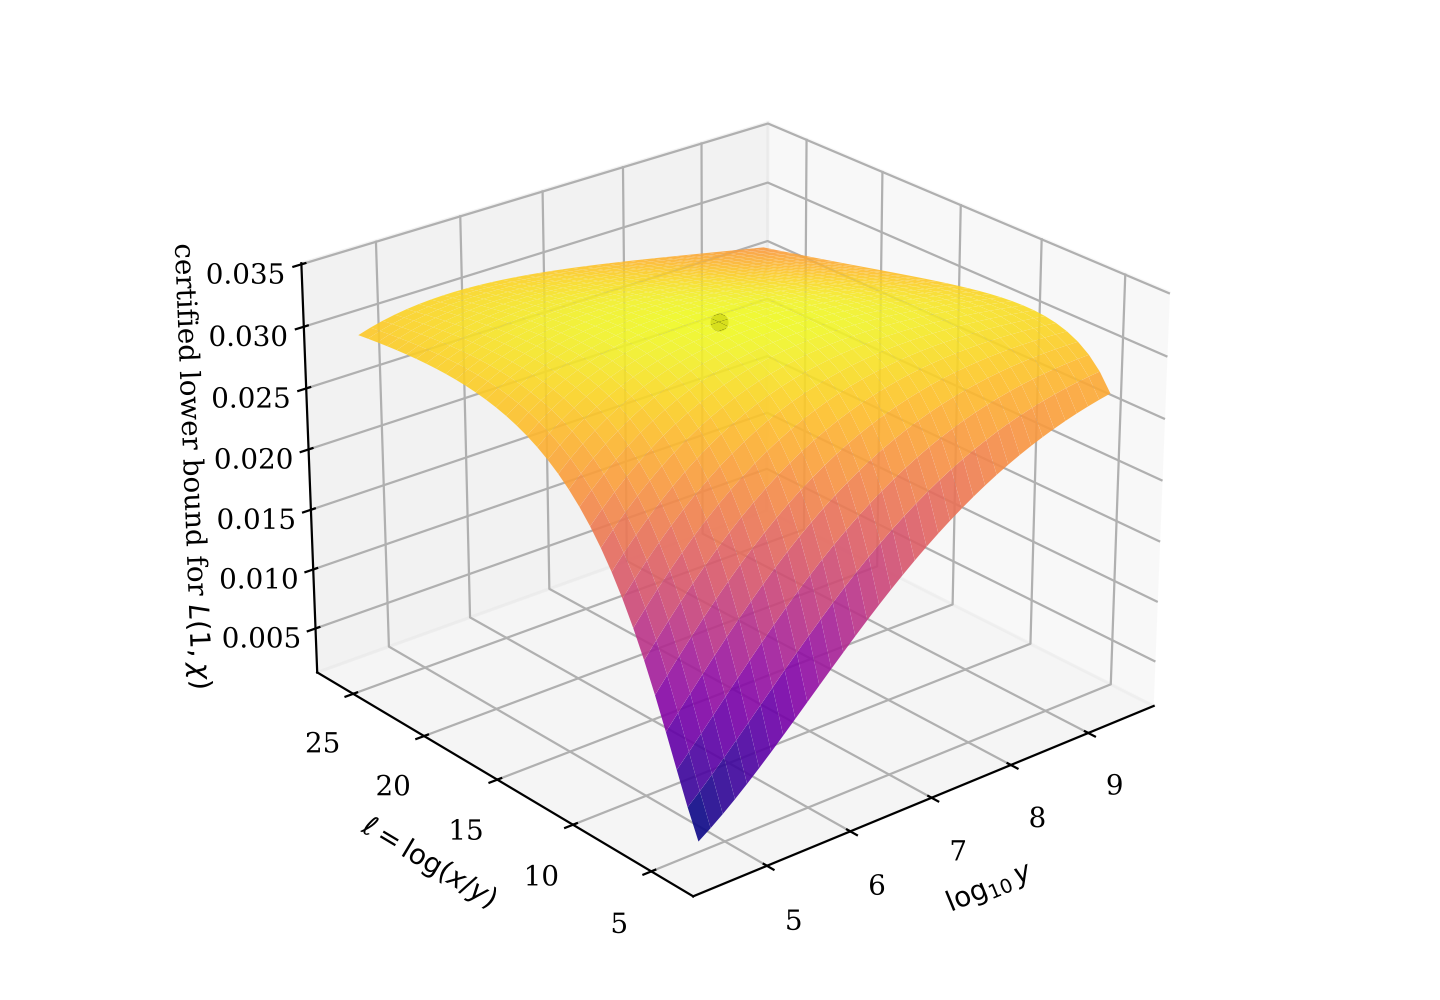
\includegraphics[width=0.78\textwidth]{figures/fig_surface.png}
\caption{The certified lower bound for $L(1,\chi)$ at $q=2^{40}$ given by Theorem~\ref{thm:general} under $\mathrm H(7/8)$, as a function of $\log_{10}y$ and $\ell$, at $u=1/10$. The maximum, $0.032934$, lies near $(6.65,14)$.}
\label{fig:surface}
\end{figure}

\begin{figure}[t]
\centering
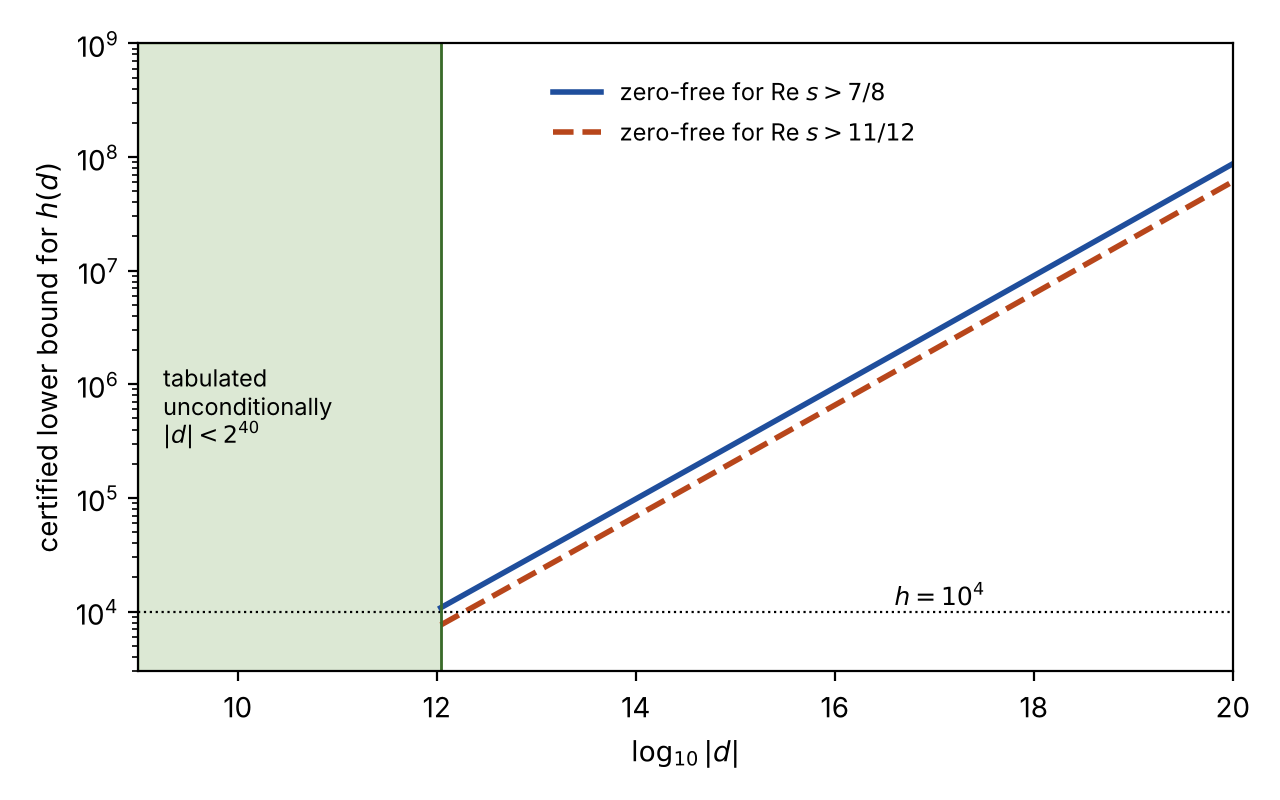
\includegraphics[width=0.82\textwidth]{figures/fig_hbound.png}
\caption{The lower bound for $h(d)$ of Theorem~\ref{thm:h} for $|d|\ge2^{40}$, from the half-planes $\Re s>7/8$ and $\Re s>11/12$. To the left of $2^{40}$ every class group is known \cite{MJ16}.}
\label{fig:hbound}
\end{figure}

\begin{remark}\label{rem:liu}
Liu's half-plane $\Re s>0.874957\ldots$ \cite{Liu26} changes the optimised bound at $q=2^{40}$ by less than $10^{-5}$. The constant that matters is $k=1/(1-B)$: as $B\to\tfrac12$ the method returns bounds of Littlewood's order with $k=2$. Explicit forms of Littlewood's bounds under the generalised Riemann hypothesis were given by Lamzouri, Li and Soundararajan \cite{LLS15}.
\end{remark}

\begin{remark}\label{rem:real}
For a real quadratic field of discriminant $d>0$ the class number formula $h(d)\log\varepsilon_d=\sqrt d\,L(1,\chi_d)/2$ and Theorem~\ref{thm:main} give $h(d)\log\varepsilon_d\ge0.36\sqrt d/(8\log\log d-4.15)$ for $d\ge2^{40}$.
\end{remark}

\section{An unconditional range with one possible exception}\label{sec:uncond}

Tatuzawa \cite[Lemma~9 and Theorem~2]{Tat51} proved the following effective form of Siegel's theorem: if $0<\varepsilon<1/11.2$, then with at most one exception every fundamental discriminant $D$ with $|D|\ge\max(e^{1/\varepsilon},e^{11.2})$ satisfies
\begin{equation}\label{eq:tatuzawa}
L(1,\chi_D)\ \ge\ 0.655\,\varepsilon\,|D|^{-\varepsilon}.
\end{equation}

\begin{proof}[Proof of Theorem~\ref{thm:uncond}]
Take $\varepsilon=1/\log(2^{40})=0.036067\ldots$, which is below $1/11.2$, so that $e^{1/\varepsilon}=2^{40}>e^{11.2}$. Let $d^*$ be the exceptional discriminant of \eqref{eq:tatuzawa} for this $\varepsilon$, if there is one. For every other fundamental $d<-2^{40}$ the class number formula and \eqref{eq:tatuzawa} give
\[
h(d)=\frac{\sqrt{|d|}\,L(1,\chi_d)}{\pi}\ \ge\ \frac{0.655\,\varepsilon}{\pi}\,|d|^{1/2-\varepsilon}\ \ge\ \frac{0.655\,\varepsilon}{\pi}\,\bigl(2^{40}\bigr)^{1/2-\varepsilon}=\frac{0.655\cdot2^{20}}{e\,\pi\log 2^{40}}=2900.757\ldots,
\]
because $1/2-\varepsilon>0$ and $(2^{40})^{-\varepsilon}=e^{-1}$. Hence $h(d)\ge2901$. If $h\le2900$ and $d\ne d^*$ has class number $h$, then $|d|<2^{40}$, and the argument of Corollary~\ref{cor:cnp}, which uses only \cite{MJ16} once $|d|<2^{40}$ is known, gives $|d|\le(\pi h/0.1706)^2$. For $h\le1000$ this is the range counted in Theorem~\ref{thm:list}.
\end{proof}

The possible exception reflects a possible real zero of $L(s,\chi_{d^*})$ very close to $1$, which the hypothesis $\mathrm H(B)$ excludes. An unconditional effective bound $L(1,\chi_d)>10^4\pi/\sqrt{|d|}$ for all fundamental $d<-2^{40}$ would remove it in the range $h\le10^4$; no such bound is known, and the best unconditional effective lower bound for $h(d)$, from the method of Goldfeld, Gross and Zagier, grows only like $\log|d|$.

\section{Class numbers up to one thousand}\label{sec:forms}

Let $D>4$ and $d=-D$. A binary quadratic form $ax^2+bxy+cy^2$ with $b^2-4ac=d$ and $a>0$ is \emph{reduced} if $|b|\le a\le c$, and $b\ge0$ whenever $|b|=a$ or $a=c$. Every primitive positive definite form is properly equivalent to exactly one reduced form \cite[Theorem 2.8]{Cox13}, and the classes of primitive forms of discriminant $d$ form a group isomorphic to the class group of the order of discriminant $d$ \cite[Theorem 7.7]{Cox13}. If $d$ is fundamental then every form of discriminant $d$ is primitive, since a common factor $g>1$ of $a,b,c$ would make $d/g^2$ a discriminant. Thus for fundamental $d$,
\[
h(d)=\#\{(a,b,c)\in\mathbb Z^3:\ b^2-4ac=d,\ (a,b,c)\text{ reduced}\}.
\]
A reduced form has $3a^2\le4ac-b^2=D$, so $a\le\sqrt{D/3}$.

\begin{proof}[Proof of Theorem~\ref{thm:list}]
Let $h(d)\le1000$. By Corollary~\ref{cor:cnp}, $|d|\le(1000\pi/0.1706)^2<N:=\NBOUND$. We computed $h(d)$ for every fundamental $d$ with $|d|\le N$ by counting reduced forms: for each $a\le\sqrt{N/3}$ and $-a<b\le a$, every $c\ge a$ (with $c>a$ when $b<0$) with $4ac-b^2\le N$ adds one to the count of $D=4ac-b^2$. The discriminant $-D$ is fundamental if and only if $D\equiv3\pmod4$ and $D$ is squarefree, or $D=4m$ with $m\equiv1,2\pmod4$ and $m$ squarefree. The program and its output are in the ancillary files. The counts for $h\le100$ agree, for every $h$, with \cite{Wat04}.
\end{proof}

The computation took \TIMECOUNT{} on four cores. Within $|d|\le N$ it finds $\NFUND$ fundamental discriminants, the smallest value of $L(1,\chi_d)=\pi h(d)/\sqrt{|d|}$ being $\MINL$ at $d=\MINLD$. Figure~\ref{fig:counts} shows $F(h)$ and the largest $|d|$ against $h$.

\begin{figure}[t]
\centering
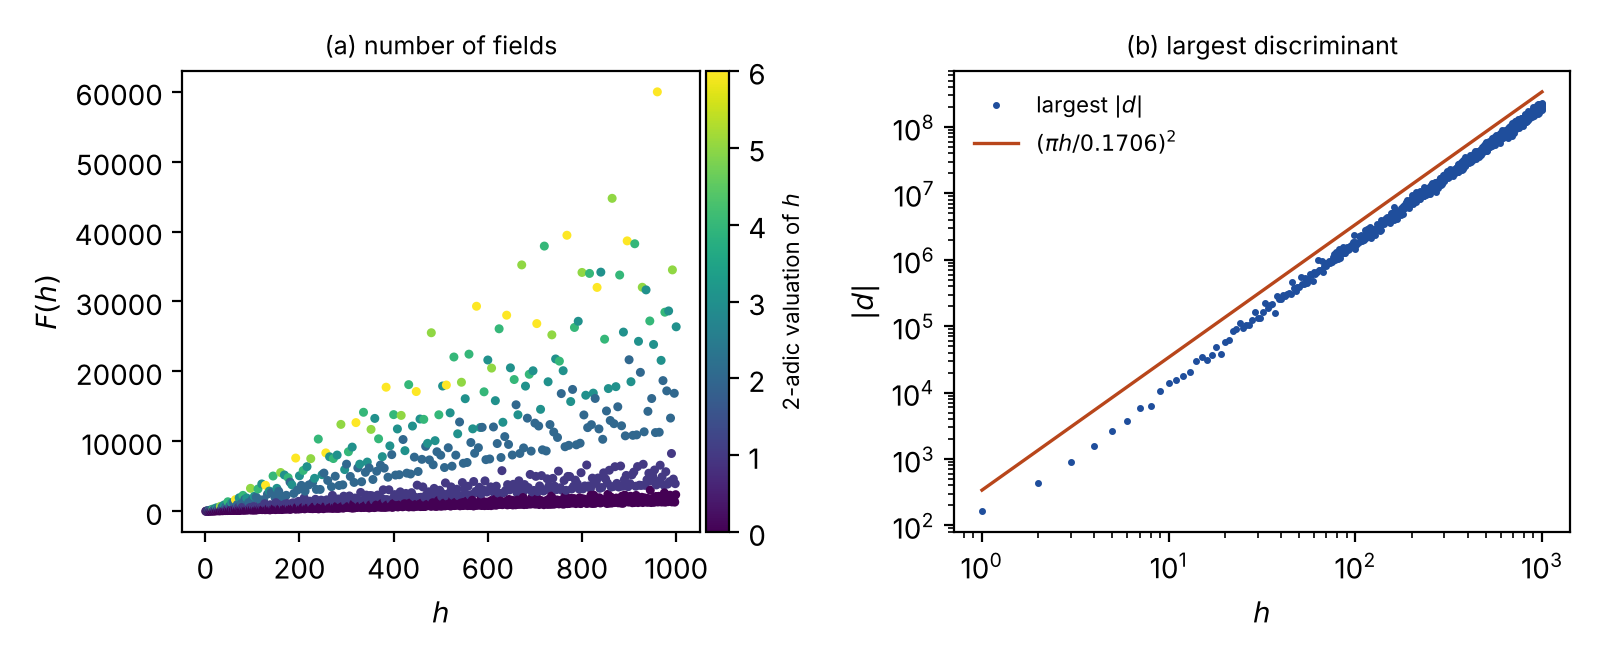
\includegraphics[width=0.95\textwidth]{figures/fig_counts.png}
\caption{(a) The number $F(h)$ of imaginary quadratic fields of class number $h$, for $h\le1000$; the upper points are the $h$ divisible by a high power of $2$. (b) The largest $|d|$ of class number $h$, with the bound $(\pi h/0.1706)^2$ of Corollary~\ref{cor:cnp}.}
\label{fig:counts}
\end{figure}

\begin{remark}
For $1000<h\le10\,798$ the same counting is possible in principle, but $|d|$ then reaches $3.9\cdot10^{10}$, and the number of operations grows like $N^{3/2}$. Corollary~\ref{cor:cnp} shows that the answer is contained in the tabulation of Mosunov and Jacobson \cite{MJ16}, which covers $|d|<2^{40}$ with all class groups computed unconditionally.\footnote{For $d\not\equiv1\pmod8$ they use class number formulas for theta series; for $d\equiv1\pmod 8$ they use the batch verification of Jacobson, Ramachandran and Williams, based on the Eichler--Selberg trace formula, which removes the dependence on the extended Riemann hypothesis.}
\end{remark}

\begin{remark}
The Riemann hypothesis itself is not touched by this work. It would replace $k=8$ by $k=2$ in Theorem~\ref{thm:main}. Any unconditional zero-free half-plane $\Re s>B$ with $B<1$ makes all results of this paper unconditional, with the constants of Theorem~\ref{thm:uniform} for that $B$.
\end{remark}

\appendix

\section{The contour argument}\label{app:contour}

We justify the shift of contour in Lemma~\ref{lem:explicit}. Put $s=1+u$ and write $s'=s+w$. We use three facts \cite[Chapters 9, 12, 16, 17 and 19]{Dav80}, together with $|\frac{L'}{L}(\sigma+it,\chi)|\le-\frac{\zeta'}{\zeta}(2)$ for $\sigma\ge2$.
\begin{enumerate}
\item For each $j\ge2$ there is $T_j\in[j,j+1]$ such that $|\frac{L'}{L}(\sigma+iT_j,\chi)|\ll\log^2(qT_j)$ uniformly for $-1\le\sigma\le2$; the same holds for $-T_j$.
\item For $\sigma\le-1$ and $s'$ at distance at least $\tfrac12$ from every trivial zero, $|\frac{L'}{L}(s',\chi)|\ll\log(q|s'|)$, by the functional equation and Stirling's formula.
\item The number of zeros with $|\gamma-t|\le1$ is $O(\log(q(|t|+2)))$.
\end{enumerate}
Let $m\ge1$ and let $\mathcal R$ be the rectangle with vertices $1\pm iT_j$ and $-U_m\pm iT_j$, where $U_m=s+2m+a+1$, so that the left side lies on $\Re s'=-2m-a-1$, midway between two trivial zeros. By the residue theorem the integral over the right side of $\mathcal R$ equals the sum of the residues inside $\mathcal R$ plus the integrals over the other three sides. On the horizontal sides, $|x^w/w^2|\le x^{\Re w}/T_j^2$ and, by (1), (2) and the bound for $\sigma\ge2$, $|\frac{L'}{L}(s',\chi)|\ll\log^2(q(T_j+U_m+2))$; the contribution is
\[
\ll\frac{\log^2(q(T_j+U_m+2))}{T_j^2}\int_{-\infty}^1x^{v}\,dv\ll\frac{x\log^2(q(T_j+U_m+2))}{T_j^2\log x}\longrightarrow0\qquad(j\to\infty,\ m\text{ fixed}).
\]
On the left side, (2) gives the bound
\[
\ll x^{-U_m}\int_{-\infty}^\infty\frac{\log(q(U_m+|t|+2))}{U_m^2+t^2}\,dt\ll x^{-U_m}\frac{\log(qU_m)}{U_m}\longrightarrow0\qquad(m\to\infty).
\]
Letting first $j\to\infty$ and then $m\to\infty$, and using (3) and $|\rho-s|\ge|\rho-1|$ to see that the sum of residues at the nontrivial zeros converges absolutely, we obtain \eqref{eq:explicit}.

\section{Certified constants}\label{app:numerics}

All constants were computed with the ball arithmetic of Arb \cite{Joh17} through python-flint at $128$ bits; every reported digit is guaranteed. The prime sum $G(10^6)$ is a sum of $78\,498$ terms evaluated in balls. The values $\zeta'/\zeta(1+u)$ and $\psi(1+u/2)$ come from the Arb series and digamma functions. The quantities entering Theorem~\ref{thm:uniform} are given below.

\begin{center}
\begin{tabular}{@{}lll@{}}
\toprule
 & $B=7/8$ & $B=11/12$\\
\midrule
$q_0,\ y_0,\ \ell,\ u$ & $2^{40},\ 5\cdot10^6,\ 14,\ 0.1$ & $2^{40},\ 1.8\cdot10^9,\ 20,\ 0.08$\\
$k$ & $8$ & $12$\\
$S(q_0,u,B)$ & $323.75077\ldots$ & $587.32747\ldots$\\
$c_0$ & $8.61975\ldots$ & $11.10846\ldots$\\
$E_0$ & $0.2378758\ldots$ & $0.2560657\ldots$\\
$3/\sqrt{y_0}$ & $0.0013416\ldots$ & $0.0000707\ldots$\\
$\kappa_0$ & $-4.1539838\ldots$ & $-8.5573459\ldots$\\
$C_-$ & $0.7255435\ldots$ & $0.7140854\ldots$\\
$C_+$ & $2.2671750\ldots$ & $2.3035538\ldots$\\
lower bound for $L(1,\chi)$ at $q_0$ & $0.0323543\ldots$ & $0.0228062\ldots$\\
lower bound for $h(d)$, $|d|\ge q_0$ & $10\,798.96\ldots$ & $7\,612.07\ldots$\\
\bottomrule
\end{tabular}
\end{center}

\noindent Here $G(10^6)=0.18198181652902\ldots$, $B_1=0.26149721284764\ldots$ and $\gamma=0.57721566490153\ldots$.

\section{Class numbers up to one thousand}\label{app:data}

The table lists, for selected $h$, the number $F(h)$ of imaginary quadratic fields of class number $h$ and the largest $|d|$ among them. The values for every $h\le1000$ are in the ancillary file \texttt{classnumbers\_1000.txt}, together with the program that produces them.

\begin{center}\small
\begin{tabular}{@{}rrr@{\qquad}rrr@{\qquad}rrr@{}}
\toprule
$h$ & $F(h)$ & max $|d|$ & $h$ & $F(h)$ & max $|d|$ & $h$ & $F(h)$ & max $|d|$\\
\midrule
1 & 9 & 163 & 28 & 457 & 126\,043 & 400 & 13\,823 & 32\,492\,923\\
2 & 18 & 427 & 29 & 83 & 166\,147 & 425 & 845 & 35\,307\,787\\
3 & 16 & 907 & 30 & 255 & 134\,467 & 450 & 3\,745 & 40\,868\,683\\
4 & 54 & 1\,555 & 31 & 73 & 133\,387 & 475 & 961 & 43\,078\,963\\
5 & 25 & 2\,683 & 32 & 708 & 164\,803 & 500 & 8\,023 & 53\,698\,747\\
6 & 51 & 3\,763 & 33 & 101 & 222\,643 & 525 & 1\,630 & 51\,065\,683\\
7 & 31 & 5\,923 & 34 & 219 & 189\,883 & 550 & 3\,254 & 69\,758\,203\\
8 & 131 & 6\,307 & 35 & 103 & 210\,907 & 575 & 1\,126 & 61\,595\,227\\
9 & 34 & 10\,627 & 36 & 668 & 217\,627 & 600 & 21\,632 & 72\,789\,403\\
10 & 87 & 13\,843 & 37 & 85 & 158\,923 & 625 & 1\,140 & 81\,289\,723\\
11 & 41 & 15\,667 & 38 & 237 & 289\,963 & 650 & 3\,683 & 85\,527\,187\\
12 & 206 & 17\,803 & 39 & 115 & 253\,507 & 675 & 1\,973 & 104\,367\,187\\
13 & 37 & 20\,563 & 40 & 912 & 260\,947 & 700 & 12\,611 & 96\,016\,243\\
14 & 95 & 30\,067 & 50 & 345 & 389\,467 & 725 & 1\,301 & 106\,911\,667\\
15 & 68 & 34\,483 & 75 & 237 & 916\,507 & 750 & 5\,750 & 113\,620\,123\\
16 & 322 & 31\,243 & 100 & 1\,736 & 1\,856\,563 & 775 & 1\,443 & 134\,009\,467\\
17 & 45 & 37\,123 & 125 & 290 & 2\,944\,363 & 800 & 34\,149 & 129\,667\,987\\
18 & 150 & 48\,427 & 150 & 1\,233 & 4\,163\,443 & 825 & 2\,305 & 130\,788\,067\\
19 & 47 & 38\,707 & 175 & 450 & 4\,742\,467 & 850 & 4\,633 & 135\,386\,227\\
20 & 350 & 58\,507 & 200 & 5\,081 & 7\,206\,763 & 875 & 1\,801 & 149\,457\,163\\
21 & 85 & 61\,483 & 225 & 709 & 9\,119\,203 & 900 & 21\,669 & 180\,619\,363\\
22 & 139 & 85\,507 & 250 & 1\,472 & 12\,208\,267 & 925 & 1\,579 & 164\,446\,027\\
23 & 68 & 90\,787 & 275 & 628 & 14\,420\,323 & 950 & 5\,087 & 186\,089\,443\\
24 & 511 & 111\,763 & 300 & 6\,744 & 19\,184\,323 & 975 & 2\,638 & 184\,039\,507\\
25 & 95 & 93\,307 & 325 & 691 & 19\,385\,683 & 1000 & 26\,378 & 220\,287\,043\\
26 & 190 & 103\,027 & 350 & 2\,258 & 24\,669\,283 &  &  & \\
27 & 93 & 103\,387 & 375 & 1\,099 & 26\,809\,843 &  &  & \\
\bottomrule
\end{tabular}
\end{center}


\section*{Declarations}

\subsection*{Data availability} The programs (interval-arithmetic bounds in Python with python-flint, and the reduced-form counter in C with OpenMP) and the output for $h\le1000$ are included as ancillary files and archived with the source of this paper at doi:10.5281/zenodo.24124876.

\subsection*{Funding} No funding was received for this work.

\subsection*{Conflict of interest} The author declares no conflict of interest.

\subsection*{Ethics} Not applicable; the work involves no human or animal subjects.

\subsection*{Use of artificial intelligence} AI coding assistants were used to write and test the computer programs and to check the bibliography. All mathematical arguments were written and verified by the author, who takes full responsibility for the content.

\begin{thebibliography}{99}\raggedright

\bibitem{Bak66} A.~Baker, \emph{Linear forms in the logarithms of algebraic numbers}, Mathematika \textbf{13} (1966), 204--216. doi:10.1112/S0025579300003971.

\bibitem{Cox13} D.~A.~Cox, \emph{Primes of the form $x^2+ny^2$}, 2nd ed., Wiley, Hoboken, NJ, 2013. doi:10.1002/9781118400722.

\bibitem{Dav80} H.~Davenport, \emph{Multiplicative number theory}, 2nd ed., revised by H.~L.~Montgomery, Graduate Texts in Mathematics \textbf{74}, Springer, New York, 1980. doi:10.1007/978-1-4757-5927-3.

\bibitem{Gol85} D.~Goldfeld, \emph{Gauss' class number problem for imaginary quadratic fields}, Bull. Amer. Math. Soc. (N.S.) \textbf{13} (1985), 23--37. doi:10.1090/S0273-0979-1985-15352-2.

\bibitem{GZ86} B.~H.~Gross and D.~B.~Zagier, \emph{Heegner points and derivatives of $L$-series}, Invent. Math. \textbf{84} (1986), 225--320. doi:10.1007/BF01388809.

\bibitem{Hee52} K.~Heegner, \emph{Diophantische Analysis und Modulfunktionen}, Math. Z. \textbf{56} (1952), 227--253. doi:10.1007/BF01174749.

\bibitem{Joh17} F.~Johansson, \emph{Arb: efficient arbitrary-precision midpoint-radius interval arithmetic}, IEEE Trans. Comput. \textbf{66} (2017), 1281--1292. doi:10.1109/TC.2017.2690633.

\bibitem{LLS15} Y.~Lamzouri, X.~Li and K.~Soundararajan, \emph{Conditional bounds for the least quadratic non-residue and related problems}, Math. Comp. \textbf{84} (2015), 2391--2412. doi:10.1090/S0025-5718-2015-02925-1.

\bibitem{Lit28} J.~E.~Littlewood, \emph{On the class-number of the corpus $P(\sqrt{-k})$}, Proc. London Math. Soc. (2) \textbf{27} (1928), 358--372. doi:10.1112/plms/s2-27.1.358.

\bibitem{Liu26} B.~Liu, \emph{Improved zero-free half-planes for the quasi-Riemann hypothesis}, arXiv:2610.12234 (2026).

\bibitem{MV07} H.~L.~Montgomery and R.~C.~Vaughan, \emph{Multiplicative number theory I. Classical theory}, Cambridge Studies in Advanced Mathematics \textbf{97}, Cambridge University Press, 2007. doi:10.1017/CBO9780511618314.

\bibitem{MJ16} A.~S.~Mosunov and M.~J.~Jacobson, Jr., \emph{Unconditional class group tabulation of imaginary quadratic fields to $|\Delta|<2^{40}$}, Math. Comp. \textbf{85} (2016), 1983--2009. doi:10.1090/mcom3050.

\bibitem{OAI-QRH} OpenAI, \emph{The quasi-Riemann hypothesis: a zero-free half-plane $\Re s>7/8$}, OpenAI Math Release preprint, 30 September 2026, \url{https://github.com/openai/math}, commit adc7f12.

\bibitem{OAI-1112} OpenAI, \emph{The quasi-Riemann hypothesis} (the half-plane $\Re s>11/12$), OpenAI Math Release preprint, 5 October 2026, \url{https://github.com/openai/math}, commit adc7f12.

\bibitem{OAI-family} OpenAI, \emph{Lean formalisation of the Dirichlet $L$-function half-plane $\Re s>7/8$} (file \texttt{DirichletSevenEighths.lean}), \url{https://github.com/openai/math}, commit adc7f12.

\bibitem{RS62} J.~B.~Rosser and L.~Schoenfeld, \emph{Approximate formulas for some functions of prime numbers}, Illinois J. Math. \textbf{6} (1962), 64--94. doi:10.1215/ijm/1255631807.

\bibitem{Sie35} C.~L.~Siegel, \emph{\"Uber die Classenzahl quadratischer Zahlk\"orper}, Acta Arith. \textbf{1} (1935), 83--86. doi:10.4064/aa-1-1-83-86.

\bibitem{Sta67} H.~M.~Stark, \emph{A complete determination of the complex quadratic fields of class-number one}, Michigan Math. J. \textbf{14} (1967), 1--27. doi:10.1307/mmj/1028999653.

\bibitem{Tat51} T.~Tatuzawa, \emph{On a theorem of Siegel}, Japan. J. Math. \textbf{21} (1951), 163--178. doi:10.4099/jjm1924.21.0\_163.

\bibitem{Wat04} M.~Watkins, \emph{Class numbers of imaginary quadratic fields}, Math. Comp. \textbf{73} (2004), 907--938. doi:10.1090/S0025-5718-03-01517-5.

\end{thebibliography}

\end{document}
